\section{PingProbe: Application Fingerprint} \label{PingProbe}
\subsection{PRI Outliers}
%Observation of PRI outliers
In \Cref{Sec:DistinguishDevice}  we mentioned the phenomenon that processor occupied by other tasks may prolong the PRI as illustrated in  \Cref{PingProbeExample}. Extracting these outliers on a CC2538 running Helloworld example using threshold of $\geq 11$ms, we show the distribution of these prolonged PRIs in \Cref{PingProbeOutliers}. The histogram suggests the distribution has a strong discrete tendency, with multiple spikes presented in the graph.

\AddFigure{fig/helloworld_cc2538_outlier.png}{Histogram of PRI Outliers on CC2538 running Helloworld Example, using bins of $10$ms}{PingProbeOutliers}

We suppose the cause of such discreteness is that the delay is indeed caused by context switching in the kernel; therefore the impact of remaining time for the current task is indeed negligible. We further suppose the existence of multiple spikes is the result of switching from different contexts take different amounts of time. However, due to practical reasons, we found it difficult to experimentally confirm these hypothesises. Nevertheless, we consider this result as a strong indication that different states of the processor would result into different value of PRI, as illustrated in \Cref{PingProbeTheory}.

\begin{figure}[ht!]
	\center
	\begin{subfigure}{0.8\textwidth}
	{
		\center
		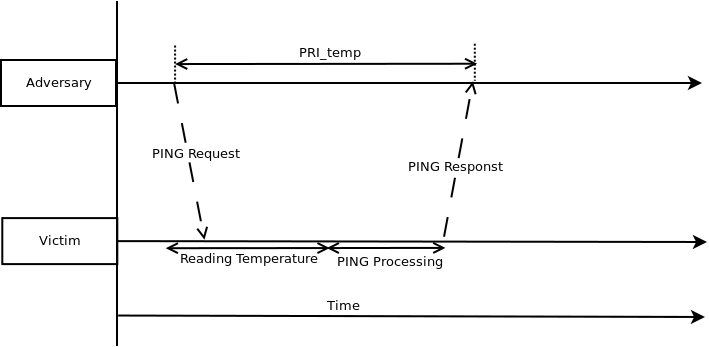
\includegraphics[width=\textwidth]{fig/PingProbe_temperature.png}
	}
	\subcaption{PRI when reading temperature sensor}
	\end{subfigure}
	\begin{subfigure}{0.8\textwidth}
	{
		\center
		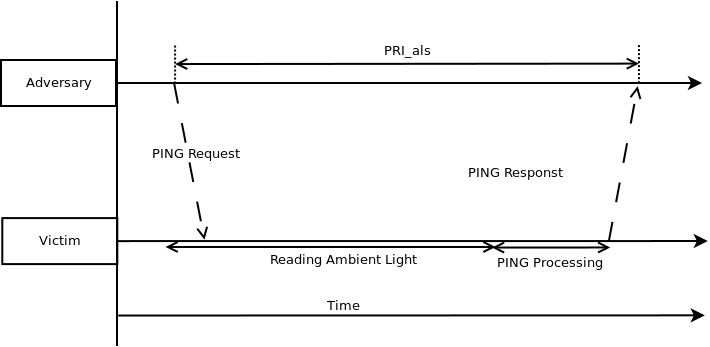
\includegraphics[width=\textwidth]{fig/PingProbe_als.png}
		\subcaption{PRI when reading Ambient Light Sensor(ALS)}
	}
	\end{subfigure}
	\caption{An example of reading temperature and ALS sensor results into different PRI.}
	\label{PingProbeTheory}
\end{figure}

\subsection{PingProbe Attack}
%What is PingProbe
The PingProbe attack is proposed to exploit the distribution of PRI outliers as an indicator of different states of the processor. Considering the fact that many IoT applications perform routine operations, e.g. reading temperature sensor periodically, the constitution of processor states can be effectively viewed as a fingerprint to the application running on the node. 

To verify the effectiveness of this attack, we performed a proof of concept experiment.

\subsubsection{Experiment Design}

Similar to many Traffic Analysis literature, we adopted the ``closed world'' setting for the experiment. Formally, our experiment simulates the following scenario:
\begin{itemize}
 \item The adversary is given the pre-knowledge of $n$ potential candidate applications, denote as $\mathbb{A} = \{A_1, A_2, ..., A_n\}$, and a target node running an unknown application $A_{x^*}$ where $A_{x^*} \in \mathbb{A}$. The adversary is also given the exact same hardware of target as well as the power to send PING packets to the target.
 \item The adversary eventually outputs $x$ as the guess of $x^*$. The attack is considered effective if $P(x = x^*) > \frac{1}{n}$.
\end{itemize}

In reality, such scenario can be motivated as an adversary trying to find out which product a victim might be using among those available on the market.

\subsubsection{Attack Description \label{PingProbeAttackManual}} 

The attack can be described into 3 stages:

\begin{description}
	\item[Profiling]
	To set up the attack, the adversary collects PRIs for each application in $\mathbb{A}$. We denote the profiled traces as:
	\begin{equation}
		\mathbb{T}_p = \{T_1, T_2, ..., T_n\}
	\end{equation}
where each $T_i$ is collected by repetitively sending PING Request to the device running application $A_i$. Each trace $T_i$ contains multiple PRIs, denote as:
	\begin{equation}
		T_i = \{t_{(i,1)}, t_{(i,2)}, ..., t_{(i,{m_i})}\} %\text{ for } i \in [1,n]
	\end{equation}
	where $m_i$ is the number of PRIs in $T_i$.

	\item[Collecting Target Trace]
	To identify the secret application $A_{x^*}$, the adversary collects the PRIs on the target node running $A_{x^*}$. We denote the target trace as:
	\begin{equation}
		T_{x^*} = \{ t_{(x^*,1)}, t_{(x^*,2)}, ..., t_{(x^*,{m_x})}\} % PRI_^x_1, $%PRI^x_2, ..., PRI^x_{m_x}\}$.
	\end{equation}
	
	\item[Matching Fingerprint]
	The first step of matching fingerprint is to filter out the outliers in each trace by a threshold $\alpha$. In practice, such threshold can be easily determined from a trace. For example, for the data we have shown in \Cref{PRIs}, $11$ms is a reasonable choice of $\alpha$ for CC2538, as most PRIs are within the range of $[9,10.5]$(ms).
	
	We then filter each trace in $\mathbb{T}$ by keeping only PRIs $\geq \alpha$:
	\begin{equation}
		T^{\prime}_{i} = \{t \in T_i | t \geq \alpha\}
	\end{equation}
	
	We denote the set of filtered profiling traces as:
	\begin{equation}
		\mathbb{T}^{\prime}_{p} = \{ T^{\prime}_1, T^{\prime}_2, ..., T^{\prime}_n\}
	\end{equation}
	Indeed the filtering of profiled traces could also be pre-computed.
	
	We then apply the same filter on target trace:
	\begin{equation}
		T^{\prime}_{x^*} =  \{t \in T_{x^*} | t > \alpha\}
	\end{equation}
	
	The adversary then searches for $T^{\prime}_{x} \in \mathbb{T}^{\prime}_p$ that is statistically most similar to $T^{\prime}_{x^*}$. One way is to use Kolmogorov-Smirniov Distance (KS distance) as the measurement of statistical similarity. The adversary then  outputs the index of the trace with minimum KS-distance to the target, i.e. to search $T^{\prime}_x$ such that:
	\begin{equation}
		KSD( T^{\prime}_{x}, T^{\prime}_{x^*}) = min(\{KSD(T^{\prime}_i, T^{\prime}_{x^*}) | i \in [1,n]\})
	\end{equation}
	where $KSD(X, Y)$ represents the KS distance between two distributions $X$ and $Y$.	Finally the adversary outputs $x$ as the guess of $x^*$.
\end{description}

\subsubsection{Experiment Result}

We performed the experiments on CC2538. The ``closed world'' includes 10 applications which are:
\begin{itemize}
	\item \textbf{powertrace}: This Contiki example continuously records the power consumption on the node.
	\item \textbf{broadcast}: This Contiki example broadcasts a test ``Test'' string periodically.
	\item \textbf{sensorpayload} family: These applications periodically read the sensors and report the readings to the root node encrypted. There are $8$ instances of this type of applications corresponding to $8$ different combinations of temperature, light and voltage sensors.
\end{itemize}

The experiments are summarised in \Cref{PingProbeExpSum}.

PING requests are sent from a Linux host with the command  ``ping6 -s 0 -i 0.4''\footnote{No user defined data and with interval of $0.4$ second}. This frequency is chosen to maximise the speed of data generation without flooding the device.

For each application, we collected $2$ packet dumps (pcapng files) with each dump consists of $200000$ packets. Traces of nearly $7000$ PRIs are extracted from each dump.

We applied the threshold $\alpha = 11\text{(ms)}$ for CC2538. Roughly 1000 PRI outliers are filtered from each trace. \Cref{PingProbeApps} summarises the data we used in the experiment.

For each trace in the experiment, there is exactly one other trace among the 20 that is collected on the same application. We applied the KS distances method as described in \Cref{PingProbeAttackManual}, as summarised in \Cref{ksdistances}.

The experiments reported 13 out of 20 ($65$\%) traces have successfully matched to the correct application in our setting.

\subsubsection{Result Analysis}

Let null hypothesis be the attack has no effect, then each trace is uniformly matched to one in the other 19 traces. 

Under the null hypothesis, the probability $P_0$ of having 13 out of 20 traces correctly matched is hence:
\begin{equation*}
P_0 = C^{13}_{20} (\frac{1}{19})^{13} (\frac{18}{19})^{7} \approx 1.262 * 10^{-12} \leq 0.01
\end{equation*}

Therefore we reject the null hypothesis and conclude that the experiments have shown positive result to the attack.